%% LyX 1.3 created this file.  For more info, see http://www.lyx.org/.
%% Do not edit unless you really know what you are doing.
\documentclass[english, 12pt]{article}
\usepackage{times}
%\usepackage{algorithm2e}
\usepackage{url}
\usepackage{bbm}
\usepackage[T1]{fontenc}
\usepackage[latin1]{inputenc}
\usepackage{geometry}
\geometry{verbose,letterpaper,tmargin=2cm,bmargin=2cm,lmargin=1.5cm,rmargin=1.5cm}
\usepackage{rotating}
\usepackage{color}
\usepackage{graphicx}
\usepackage{amsmath, amsthm, amssymb}
\usepackage{setspace}
\usepackage{lineno}
\usepackage{hyperref}
\usepackage{bbm}
\usepackage{makecell}
\usepackage{placeins}
\usepackage{subcaption}

%\renewcommand{\arraystretch}{1.8}

%\linenumbers
%\doublespacing
\onehalfspacing
%\usepackage[authoryear]{natbib}
\usepackage{natbib} \bibpunct{(}{)}{;}{author-year}{}{,}

%Pour les rajouts
\usepackage{color}
\definecolor{trustcolor}{rgb}{0,0,1}

\usepackage{dsfont}
\usepackage[warn]{textcomp}
\usepackage{adjustbox}
\usepackage{multirow}
\usepackage{subcaption}
\usepackage{graphicx}
\graphicspath{{../figures/}}
\DeclareMathOperator*{\argmin}{\arg\!\min}

\let\tabbeg\tabular
\let\tabend\endtabular
\renewenvironment{tabular}{\begin{adjustbox}{max width=0.95\textwidth}\tabbeg}{\tabend\end{adjustbox}}

\makeatletter

%%%%%%%%%%%%%%%%%%%%%%%%%%%%%% LyX specific LaTeX commands.
%% Bold symbol macro for standard LaTeX users
%\newcommand{\boldsymbol}[1]{\mbox{\boldmath $#1$}}

%% Because html converters don't know tabularnewline
\providecommand{\tabularnewline}{\\}
\renewcommand*{\arraystretch}{1.2}

\usepackage{babel}
\makeatother


\begin{document}

\renewcommand{\thefigure}{S\arabic{figure}}
\setcounter{figure}{0}
\renewcommand{\thetable}{S\arabic{table}}
\setcounter{table}{0}
\renewcommand{\theequation}{S\arabic{equation}}
\setcounter{equation}{0}

\section*{Supplementary Materials}

\vspace*{5em}


%%%%%%%%%%%%%%%%%%%%%%%%%%%%%%%%%%%%%%%%%%%%%%%%%%%%%%%%%%%%%%%%%%%%%%%%%%%%%%%%


\begin{figure}[h]
	\centerline{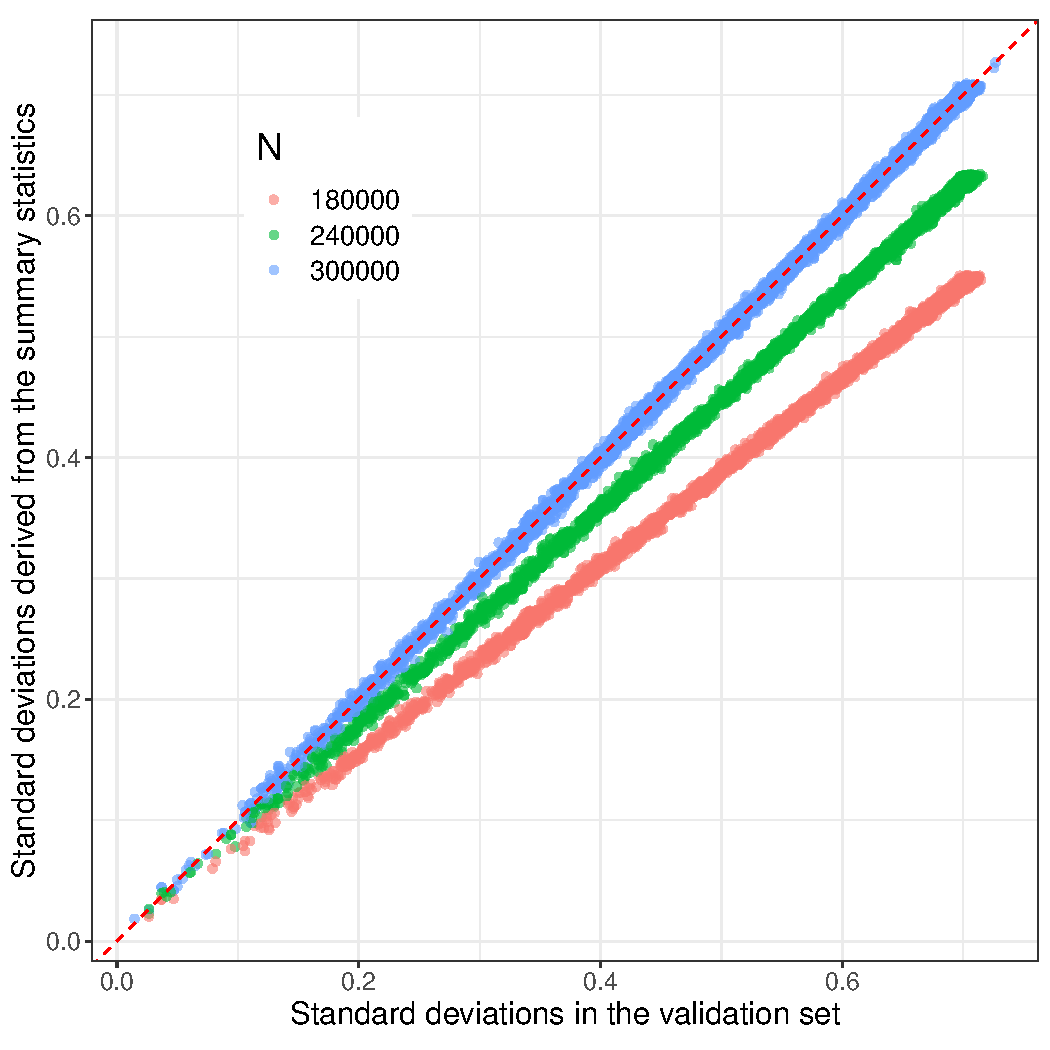
\includegraphics[width=0.8\textwidth]{simu-qc-plot}}
	\caption{Quality control plot, as proposed in \cite{prive2020ldpred2}, for the simulations with sample size misspecification. The standard deviations are derived from the summary statistics assuming the same global GWAS sample size for all variants (300,000).}
	\label{fig:qcplot}
\end{figure}


\begin{figure}[h]
	\centerline{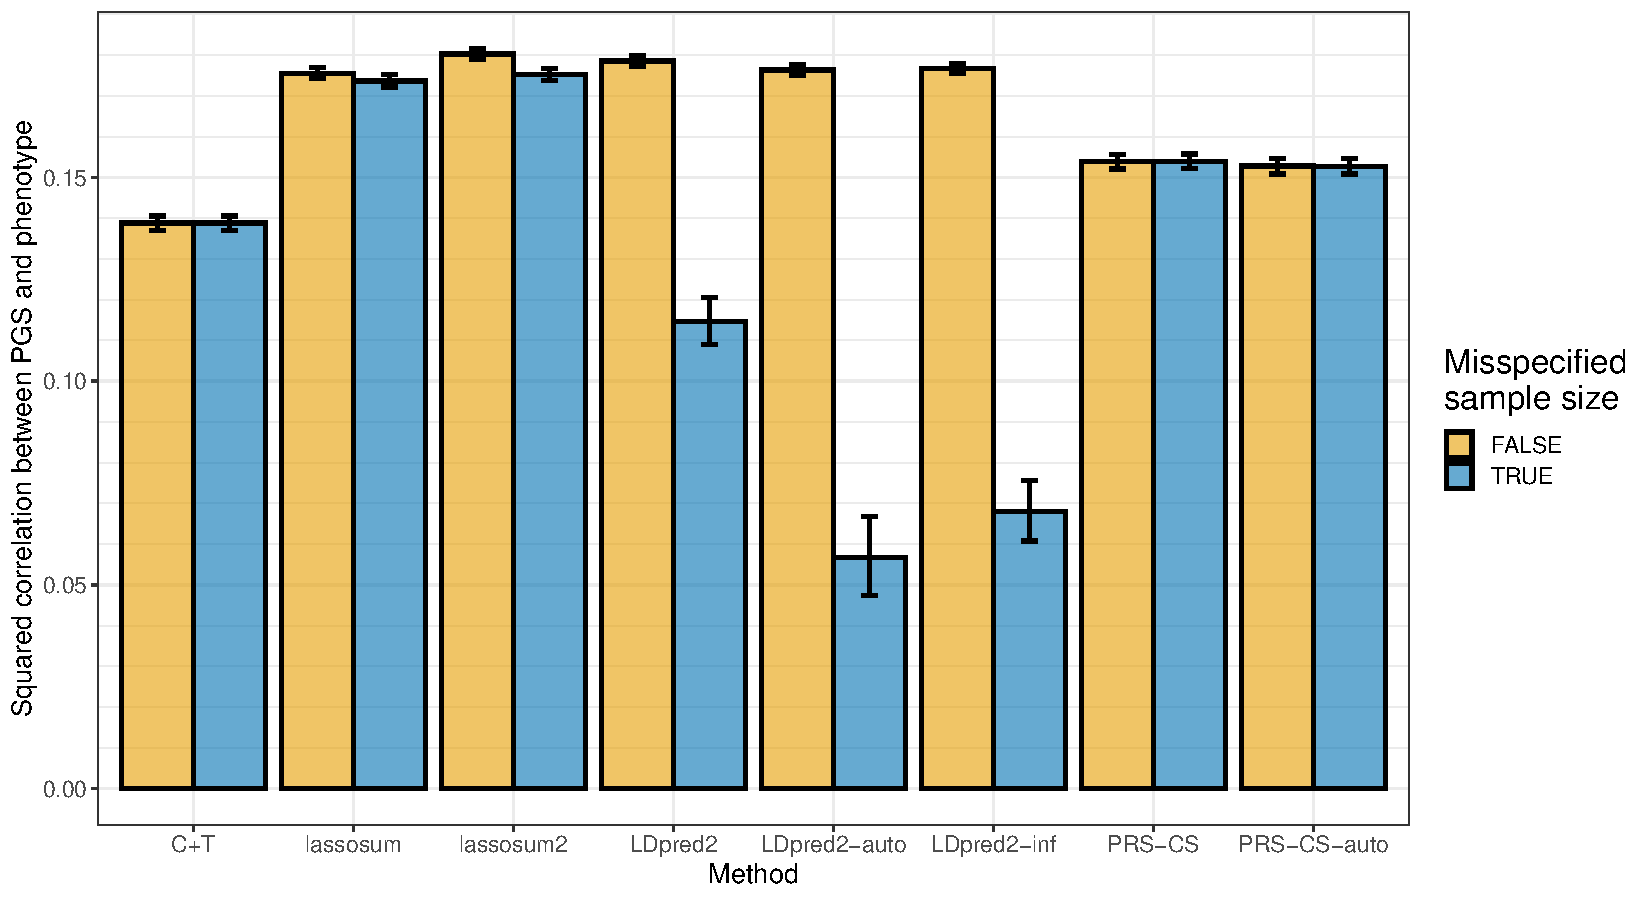
\includegraphics[width=0.95\textwidth]{simu-misN}}
	\caption{Results for the simulations with sample size misspecification. The GWAS sample size is not misspecified when providing the true per-variant sample size, and is misspecified when providing instead the maximum sample size as a unique value to be used for all variants. Note that we always use this unique total sample size for PRS-CS because it can be provided only one value. As for C+T, it never uses this information anyway, which is why we get the same predictions for these two methods in both cases of misspecification or not.}
	\label{fig:simu-misN}
\end{figure}


\begin{figure}[h]
	\centerline{\includegraphics[width=0.85\textwidth]{pseudoval}}
	\caption{For one simulation, scores from validation vs.\ scores from pseudo-validation as described in \cite{mak2017polygenic} using either correlations (the default in lassosum) or p-values for computing local false discovery rates.}
	\label{fig:pseudoval}
\end{figure}

%%%%%%%%%%%%%%%%%%%%%%%%%%%%%%%%%%%%%%%%%%%%%%%%%%%%%%%%%%%%%%%%%%%%%%%%%%%%%%%%

%\clearpage


%%%%%%%%%%%%%%%%%%%%%%%%%%%%%%%%%%%%%%%%%%%%%%%%%%%%%%%%%%%%%%%%%%%%%%%%%%%%%%%%

\FloatBarrier
%\clearpage

\bibliographystyle{natbib}
\bibliography{refs}

\end{document}
